\documentclass[tikz, border=0.2cm]{standalone}
\usetikzlibrary{positioning}
\usetikzlibrary{decorations.markings}

\begin{document}

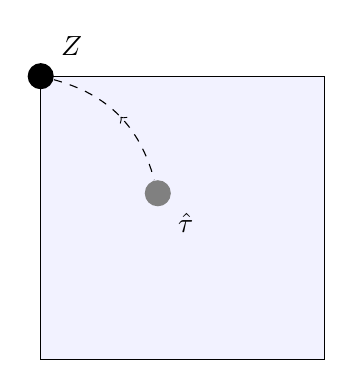
\begin{tikzpicture}

% Square
\draw[fill=blue!50!white, fill opacity=0.1] (-1.8,-1.8) rectangle (1.8,1.8);

% Anchors
\node[fill=black, circle, minimum size=1pt] (anchor1) at (-1.8,1.8) {};
\node[fill=gray, circle, minimum size=0.5pt, below right = 50pt of anchor1] (anchor2) 
{};

% Curves
\draw[-, dashed, decoration={markings, mark=at position 0.55 with {\arrow{<}}}, 
postaction={decorate}]
 (anchor1) to[bend left] (anchor2);

% Writings
\node[draw=none, fill=none, above right = 0.5pt of anchor1] (Z) {\(Z\)};
\node [draw=none, fill=none, below right = 0.5pt of anchor2] (tauhat) {\(\hat \tau\)};

\end{tikzpicture}

\end{document}
